\begin{samplecase}
{\bf Gamma-ray intensities: ${}^{208}$Pb$(n,n\gamma )$ and ${}^{208}$Pb$(n,2n\gamma )$}\newline
This feature could simply have been included in the sample case on 
excitation functions for ${}^{208}$Pb, but in order not to overburden the
description of that sample case we include it here. With the input file

\VerbatimInput{\samples n-Pb208-nngamma/org/talys.inp}

all discrete gamma lines are printed and stored in separate files.
To avoid the production of too many data files, we have put {\bf maxZ 0} so 
that only the gamma-ray production files for Pb-chain are created. Also, we 
include a special OMP with
the file {\em pb.omp} and we set {\bf isomer 1.e-4} to allow for gamma decay
of some rather short-lived levels.
Experimental data exists for 
the ${}^{208}$Pb$(n,n'\gamma)$ cross section for level 1 to level 0 and
the ${}^{208}$Pb$(n,2n'\gamma)$ cross section for level 2 to level 0 and for 
level 1 to level 0. These
data have been plotted together with the results of the calculated files
{\em gam082208L01L00.tot}, {\em gam082207L02L00.tot} and 
{\em gam082207L01L00.tot}, in Fig.~\ref{pbgamma}.
\end{samplecase}
\begin{figure}
\centering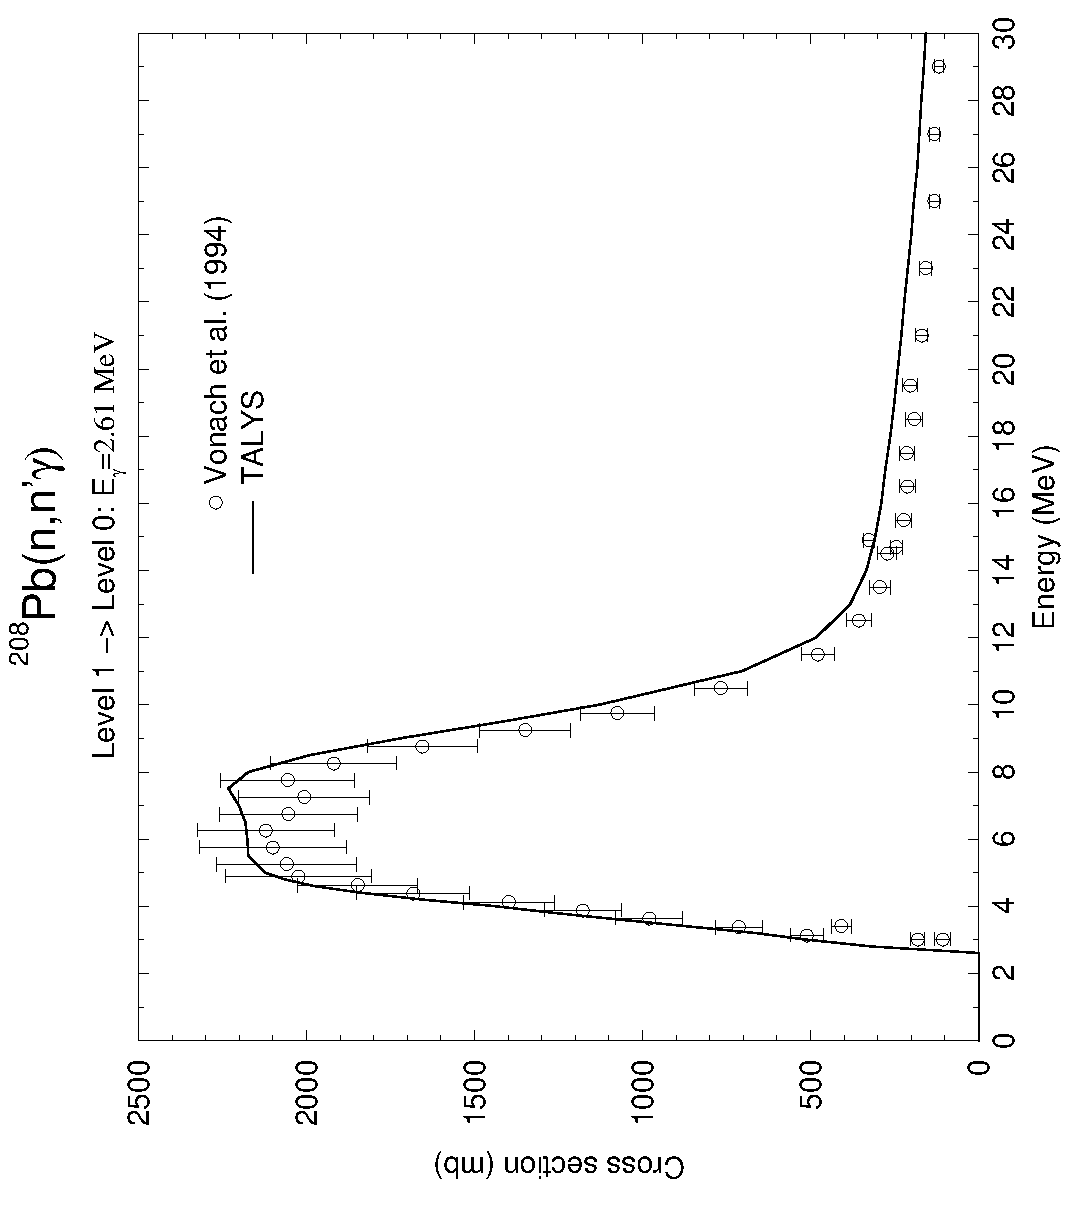
\includegraphics[scale=0.4,angle=270]{gam082208L01L00}
\centering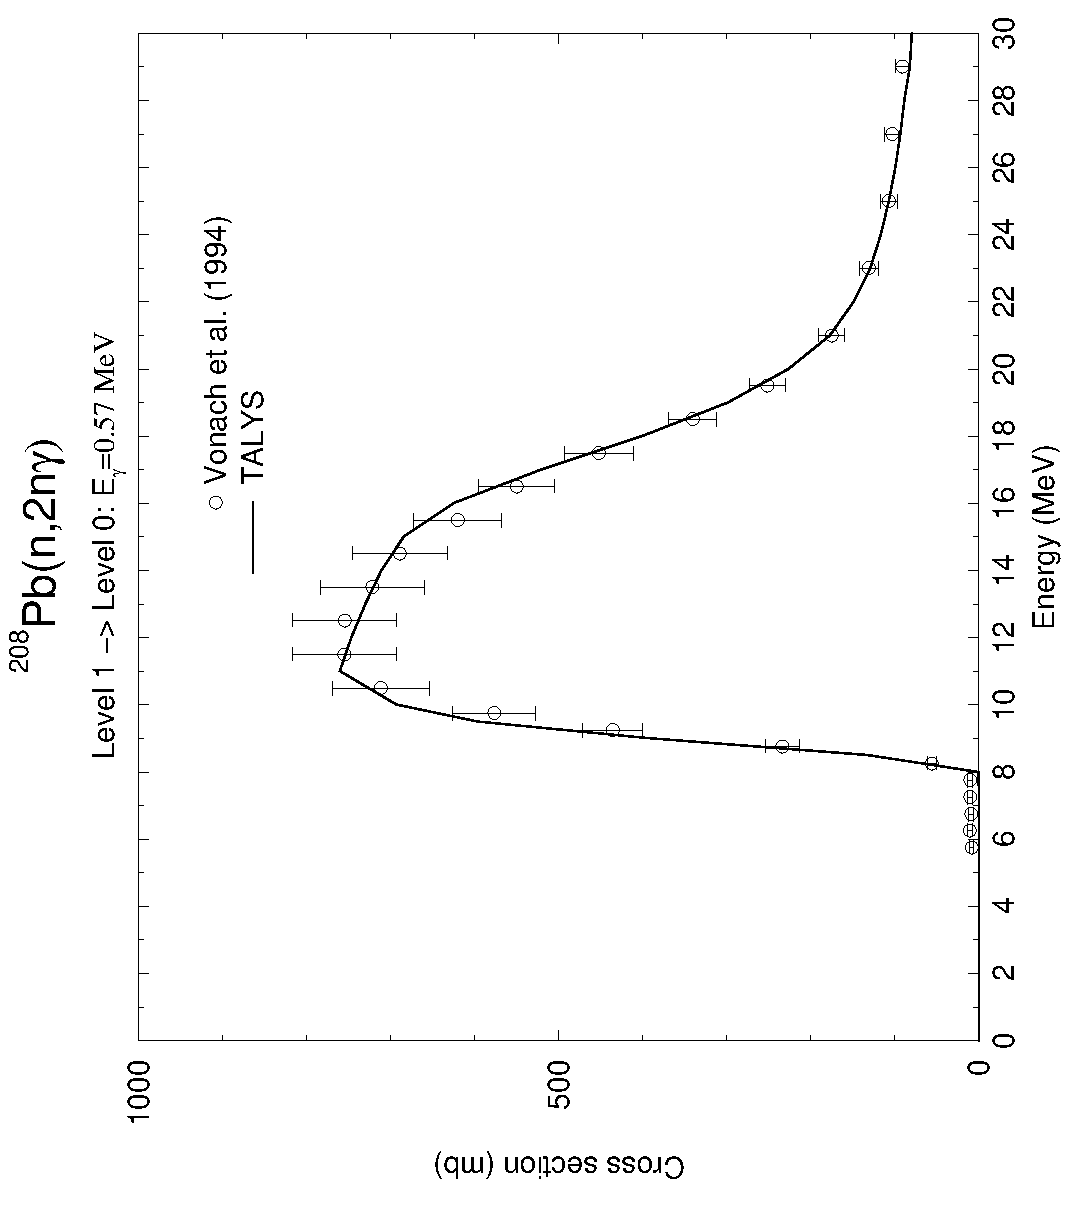
\includegraphics[scale=0.4,angle=270]{gam082207L01L00}
\centering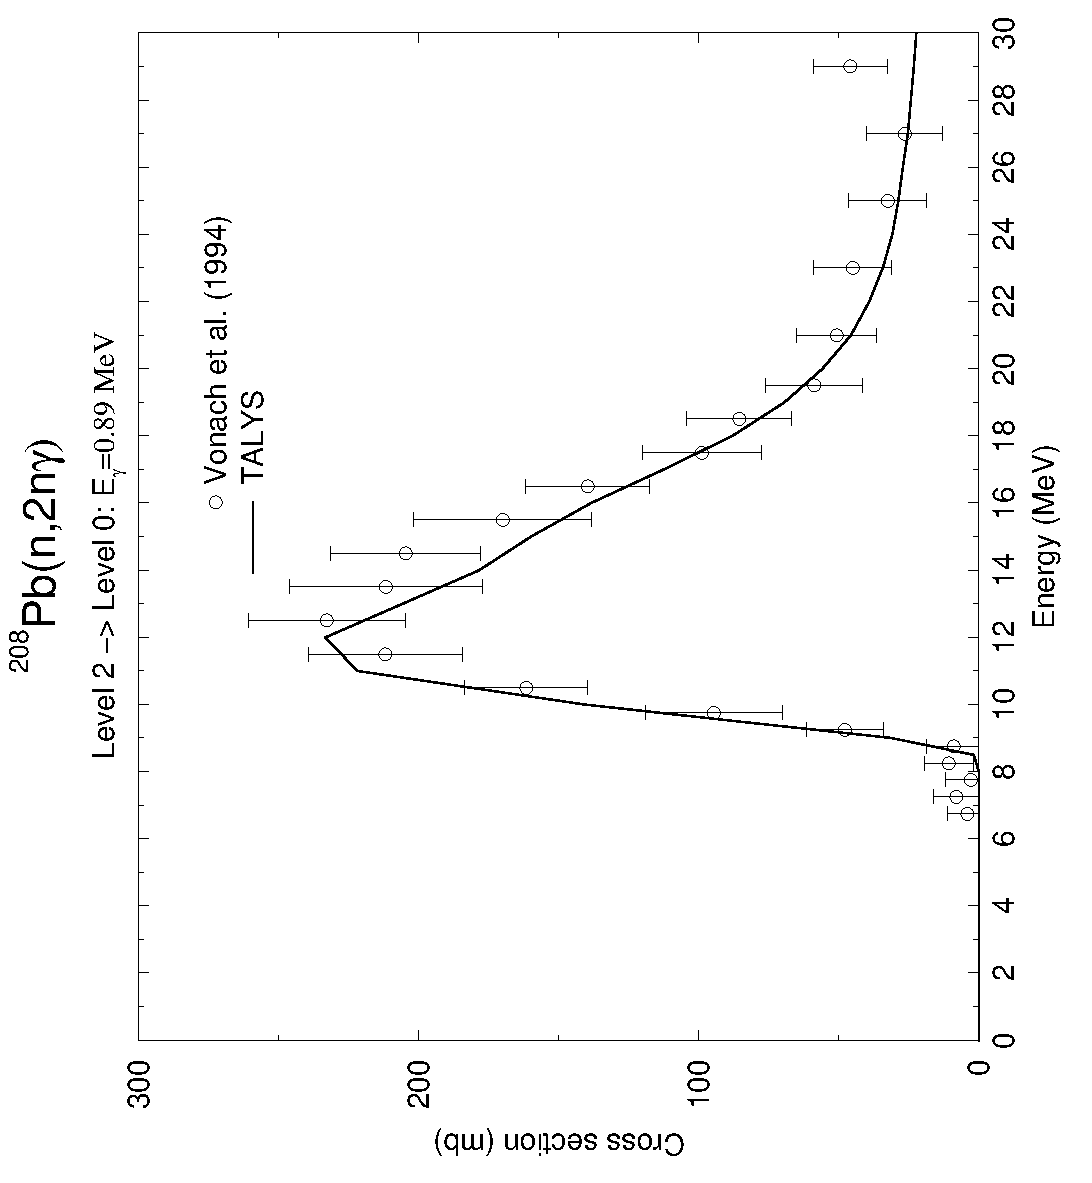
\includegraphics[scale=0.4,angle=270]{gam082207L02L00}
\caption{Gamma-ray production lines for a few transitions in ${}^{208}$Pb(n,n')
and ${}^{208}$Pb(n,2n) reactions.
The experimental data are from \protect\cite{Vonach1994}.}
\label{pbgamma}
\end{figure}
